%----------------------------------------------------------------------------------------
%	PACKAGES AND OTHER DOCUMENT CONFIGURATIONS
%----------------------------------------------------------------------------------------

\documentclass[
12pt, % The default document font size, options: 10pt, 11pt, 12pt
english, % ngerman for German
singlespacing, % Single line spacing, alternatives: onehalfspacing or doublespacing
%draft, % Uncomment to enable draft mode (no pictures, no links, overfull hboxes indicated)
%nolistspacing, % If the document is onehalfspacing or doublespacing, uncomment this to set spacing in lists to single
%liststotoc, % Uncomment to add the list of figures/tables/etc to the table of contents
%toctotoc, % Uncomment to add the main table of contents to the table of contents
%parskip, % Uncomment to add space between paragraphs
%nohyperref, % Uncomment to not load the hyperref package
headsepline, % Uncomment to get a line under the header
%chapterinoneline, % Uncomment to place the chapter title next to the number on one line
%consistentlayout, % Uncomment to change the layout of the declaration, abstract and acknowledgements pages to match the default layout
]{MastersDoctoralThesis} 

\usepackage[utf8]{inputenc} % Required for inputting international characters
\usepackage[T1]{fontenc} % Output font encoding for international characters
\usepackage{mathpazo} % Use the Palatino font by default

% Use the bibtex backend with the authoryear citation style (which resembles APA)
\usepackage[backend=bibtex,style=authoryear,natbib=true]{biblatex} 

\addbibresource{bibliografia.bib} % The filename of the bibliography

\usepackage[autostyle=true]{csquotes} % Required to generate language-dependent quotes in the bibliography

%----------------------------------------------------------------------------------------
%	MARGIN SETTINGS
%----------------------------------------------------------------------------------------

\geometry{
	paper=a4paper, % Change to letterpaper for US letter
	inner=2.5cm, % Inner margin
	outer=3.8cm, % Outer margin
	bindingoffset=.5cm, % Binding offset
	top=1.5cm, % Top margin
	bottom=1.5cm, % Bottom margin
	%showframe, % Uncomment to show how the type block is set on the page
}

%----------------------------------------------------------------------------------------
%	THESIS INFORMATION
%----------------------------------------------------------------------------------------

\thesistitle{Application of Long Short Term Memory networks for GPS 
satellite clock bias prediction}
\supervisor{Dr Hab. Romuald Kotowski} % Your supervisor's name, this is used in the title page, print it elsewhere with \supname
\examiner{} % Your examiner's name, this is not currently used anywhere in the template, print it elsewhere with \examname
\degree{Doctor of Philosophy} % Your degree name, this is used in the title page and abstract, print it elsewhere with \degreename
\author{Msc. Eng. Piotr Gny\'{s}} % Your name, this is used in the title page and abstract, print it elsewhere with \authorname
\addresses{} % Your address, this is not currently used anywhere in the template, print it elsewhere with \addressname

\subject{Computer Sciences and Tellecomunication} % Your subject area, this is not currently used anywhere in the template, print it elsewhere with \subjectname
\keywords{} % Keywords for your thesis, this is not currently used anywhere in the template, print it elsewhere with \keywordnames
\university{\href{http://www.university.com}{Polish Japanese Academy of Information Technology}} % Your university's name and URL, this is used in the title page and abstract, print it elsewhere with \univname
\department{\href{http://department.university.com}{Computer Science}} % Your department's name and URL, this is used in the title page and abstract, print it elsewhere with \deptname
\group{\href{http://researchgroup.university.com}{Robotics Laboratory}} % Your research group's name and URL, this is used in the title page, print it elsewhere with \groupname
\faculty{\href{http://faculty.university.com}{Mechanics Computer Science and Robotics}} % Your faculty's name and URL, this is used in the title page and abstract, print it elsewhere with \facname

\AtBeginDocument{
\hypersetup{pdftitle=\ttitle} % Set the PDF's title to your title
\hypersetup{pdfauthor=\authorname} % Set the PDF's author to your name
\hypersetup{pdfkeywords=\keywordnames} % Set the PDF's keywords to your keywords
}

\begin{document}

\frontmatter % Use roman page numbering style (i, ii, iii, iv...) for the pre-content pages

\pagestyle{plain} % Default to the plain heading style until the thesis style is called for the body content

%----------------------------------------------------------------------------------------
%	TITLE PAGE
%----------------------------------------------------------------------------------------

\begin{titlepage}
\begin{center}

\vspace*{.06\textheight}
{\scshape\LARGE \univname\par}\vspace{1.5cm} % University name
\textsc{\Large Doctoral Thesis}\\[0.5cm] % Thesis type

\HRule \\[0.4cm] % Horizontal line
{\huge \bfseries \ttitle\par}\vspace{0.4cm} % Thesis title
\HRule \\[1.5cm] % Horizontal line
 
\begin{minipage}[t]{0.4\textwidth}
\begin{flushleft} \large
\emph{Author:}\\
\href{http://www.johnsmith.com}{\authorname} % Author name - remove the \href bracket to remove the link
\end{flushleft}
\end{minipage}
\begin{minipage}[t]{0.4\textwidth}
\begin{flushright} \large
\emph{Supervisor:} \\
\href{http://www.jamessmith.com}{\supname} % Supervisor name - remove the \href bracket to remove the link  
\end{flushright}
\end{minipage}\\[3cm]
 
\vfill

\large \textit{A thesis submitted in fulfillment of the requirements\\ for the degree of \degreename}\\[0.3cm] % University requirement text
\textit{in the}\\[0.4cm]
\groupname\\\deptname\\[2cm] % Research group name and department name
 
\vfill

{\large \today}\\[4cm] % Date
%\includegraphics{Logo} % University/department logo - uncomment to place it
 
\vfill
\end{center}
\end{titlepage}

%----------------------------------------------------------------------------------------
%	DECLARATION QUOTATION ABSTRACT AND ACKNOWLEDGMENTS
%----------------------------------------------------------------------------------------

%----------------------------------------------------------------------------------------
%	DECLARATION PAGE
%----------------------------------------------------------------------------------------

\begin{declaration}
\addchaptertocentry{\authorshipname} % Add the declaration to the table of contents
\noindent I, \authorname, declare that this thesis titled, \enquote{\ttitle} and the work presented in it are my own. I confirm that:

\begin{itemize} 
\item This work was done wholly or mainly while in candidature for a research degree at this University.
\item Where any part of this thesis has previously been submitted for a degree or any other qualification at this University or any other institution, this has been clearly stated.
\item Where I have consulted the published work of others, this is always clearly attributed.
\item Where I have quoted from the work of others, the source is always given. With the exception of such quotations, this thesis is entirely my own work.
\item I have acknowledged all main sources of help.
\item Where the thesis is based on work done by myself jointly with others, I have made clear exactly what was done by others and what I have contributed myself.\\
\end{itemize}
 
\noindent Signed:\\
\rule[0.5em]{25em}{0.5pt} % This prints a line for the signature
 
\noindent Date:\\
\rule[0.5em]{25em}{0.5pt} % This prints a line to write the date
\end{declaration}

\cleardoublepage
%----------------------------------------------------------------------------------------
%	QUOTATION PAGE
%----------------------------------------------------------------------------------------

\vspace*{0.2\textheight}

%\noindent\enquote{\foreignlanguage{russian}{\itshape 
%Все должны быть познающими и всё должно быть предметом знания}}\bigbreak
%
%\hfill Николай Федорович Федоров

\noindent\enquote{\foreignlanguage{russian}{\itshape 
Everyone should be a scientist and everything should be a subject of research}}\bigbreak

\hfill Nikolai Fyodorovich Fyodorov

%----------------------------------------------------------------------------------------
%	ABSTRACT PAGE
%----------------------------------------------------------------------------------------

\begin{abstract}
\addchaptertocentry{\abstractname} % Add the abstract to the table of contents
Long Short Term Memory (LSTM) neural networks have prooven to be a powerfull
prediction algorithm and are used in many areas where data with time series nature 
must be predicted. In this paper it is demonstrated that it can also be used for
prediction of the Global Positioning System (GPS) satellite on-board atomic clock bias.
Results of LSTM predictions were compared with a current state of the art in 
low latency GPS clock bias prediction and it was demonstrated that approach proposed
in this work is able to provide better precision of results.
\end{abstract}

%----------------------------------------------------------------------------------------
%	ACKNOWLEDGEMENTS
%----------------------------------------------------------------------------------------

\begin{acknowledgements}
\addchaptertocentry{\acknowledgementname} % Add the acknowledgements to the table of contents
The acknowledgments and the people to thank go here, don't forget to include your project advisor\ldots
\end{acknowledgements}




%----------------------------------------------------------------------------------------
%	LIST OF CONTENTS/FIGURES/TABLES PAGES
%----------------------------------------------------------------------------------------

\tableofcontents % Prints the main table of contents

\listoffigures % Prints the list of figures

\listoftables % Prints the list of tables

%----------------------------------------------------------------------------------------
%	ABBREVIATIONS
%----------------------------------------------------------------------------------------

\begin{abbreviations}{ll} % Include a list of abbreviations (a table of two columns)

%----------------------------------------------------------------------------------------
%	ABBREVIATIONS
%----------------------------------------------------------------------------------------

\begin{abbreviations}{ll} % Include a list of abbreviations (a table of two columns)
\textbf{GNSS} & \textbf{Global} \textbf{N}avigation \textbf{S}atellite \textbf{S}ystem\\
\textbf{LAH} & \textbf{L}ist \textbf{A}bbreviations \textbf{H}ere\\
\textbf{LAH} & \textbf{L}ist \textbf{A}bbreviations \textbf{H}ere\\
\textbf{LAH} & \textbf{L}ist \textbf{A}bbreviations \textbf{H}ere\\
\textbf{LAH} & \textbf{L}ist \textbf{A}bbreviations \textbf{H}ere\\
\end{abbreviations}


\end{abbreviations}

%----------------------------------------------------------------------------------------
%	PHYSICAL CONSTANTS/OTHER DEFINITIONS
%----------------------------------------------------------------------------------------

\begin{constants}{lr@{${}={}$}l} % The list of physical constants is a three column table

% The \SI{}{} command is provided by the siunitx package, see its documentation for instructions on how to use it

Speed of Light & $c_{0}$ & \SI{2.99792458e8}{\meter\per\second} (exact)\\
%Constant Name & $Symbol$ & $Constant Value$ with units\\

\end{constants}

%----------------------------------------------------------------------------------------
%	SYMBOLS
%----------------------------------------------------------------------------------------

\begin{symbols}{lll} % Include a list of Symbols (a three column table)

$a$ & distance & \si{\meter} \\
$P$ & power & \si{\watt} (\si{\joule\per\second}) \\
%Symbol & Name & Unit \\

\addlinespace % Gap to separate the Roman symbols from the Greek

$\omega$ & angular frequency & \si{\radian} \\

\end{symbols}

%----------------------------------------------------------------------------------------
%	THESIS CONTENT - CHAPTERS
%----------------------------------------------------------------------------------------

\mainmatter % Begin numeric (1,2,3...) page numbering

\pagestyle{thesis} % Return the page headers back to the "thesis" style

% Include the chapters of the thesis as separate files from the Chapters folder
% Uncomment the lines as you write the chapters

\chapter{Introduction}
FIXME : Textwidth in cm: \printinunitsof{cm}\prntlen{\textwidth}

%==================================================================================================
\section{Motivation}
I have encountered a problem that was insipration for this work during my research in field
of mobile robotics. While my initial focus was directed more towards emergent behaviour in 
robotics and a self organizing systems I have encountered a issue with localization in marine 
robotics. With high cost of internet connection for robots operating far away from land it 
is important to be able to calculate precise position without updating data from internet.
One of issuse when working with satellite navigation system is requirement for clock bias
correction, to keep error drift to minimum readouts for both local and satellite clock must
be corrected by predicted bias. In this work I focused on prediction of errors in satellite
clocks as unlike in case of local clock those can be later reused by other people.


\chapter{Time metrology}
Aim of this chapter is to present an issue that will be dealt with in this work.
First a concept of theoretical clock will be presented alongside mathematical tools required
for it description and behavior modelling.
This is followed by a more detailed description of stability analysis which is most prominent
field of science dealing with clock behavior.
After describing theoretical clock models an attention will be given to physical implementation
of clock system with special focus on types of clocks used aboard GPS satellites.
Finally current state of the art in GPS clock bias prediction will be presented.
Intention of writing this chapter was that despite clock modelling and frequency analysis being
well known field readers with computer science might not be familiar with it.
For those well versed in frequency analysis most of this chapter can be safely skipped with 
exception of last section that focuses on state of the art in GPS clock prediction as it 
deals with issues that are more specific do described in this work.
It is important to understand that this chapter do not provide comprehensive knowledge about
described field as due to methodology used in presented work that knowledge it is not required.
For more information about clock modelling and stability analysis Handbook of Frequency Stability
Analysis is suggested as reading.


%====================================================================================================
\section{Physical clock implementation}
\label{sec:physical_clock}

%----------------------------------------------------------------------------------------------------
\subsection{Introduction to physical clock implementation}
In precise time metrology clock can refer to a single oscillator or an oscillator enseble
as well as to electronic circuit that processes signal generated by oscilator.
Most commonly used oscillator is piezoelectric quartz oscillator.
Quarts 

%----------------------------------------------------------------------------------------------------
\subsection{Principles of atomic clock design}


%====================================================================================================
\section{Mathematical clock model}
\textbf{FIXME: MAKE ALL EQUATIONS USE SAME NOTATION}
In context of pure mathematical modelling a clock is understood as a function that describes
offset between two given values for a specific point in time. One of those values is referred 
to as the reference clock and it is considered to always return correct time $T_{r}(t)=t$.
It is important to understand that in physical systems value of $t$ is not only inaccessible, as
every measurement instrument have some degree of uncertainty, but do not exists at all.
This is due to time dilatation effect, derived from special theory of relativity, that causes
time to flow differently in systems that move with velocities close to speed of the light.
This issue is dealt with by selecting most precise physical clock available as the reference
clock and modelling difference between it and other clocks, including time dilatation effects,
as their bias.
Main goal of modeling clocks is to retrieve a value of $t$, which is equal to $T_{r}(t)$, based
on value read from given clock $T_{c}(t)$. 
As relation between those clock is fully described by analyzed clock bias 
$b_{c}(t)=T_{r}(t)-T_{c}(t)$ clock model is equivalent to just a bias model.

%----------------------------------------------------------------------------------------------------
\subsection{Discrete and continuous clock models}
There are two possible approaches to mathematical clock modelling, one of them is continuous
clock model that relies on differential equation for description of its behavior.
In this approach clock bias is modeled as :
\begin{equation}
	\label{equ:continous_clock}
	b_{c}(t) = T_{r}(t_{0}) +  \int_{t_{0}}^{t} \varepsilon_{c}(\tau) d\tau ,
\end{equation}
where:
\begin{itemize}
	\item $t$ is the independent time argument,
	\item $b_{c}(t)$ is the clock bias at time $t$,
	\item $t_{0}$ is time at which clock was synchronized with reference ($b_{c}(t_{0})=0$),
	\item $T_{r}(t_{0})$ is value of reference clock at $t_{0}$,
	\item $\varepsilon_{c}(\tau)$ is the normalized frequency offset of a clock.
\end{itemize}
The branch of science that deals with continuous clock modelling is called stability analysis.
In this work no more attention will be given to that approach as due to nature of data as well as
choice of prediction algorithms favour a discrete clock model.
In discrete clock model bias is described as :
\begin{equation}
	\label{equ:discrete_clock}
	b_{c}(i) = T_{r}(i) - T_{c}(i),
\end{equation}
where $i \in \mathbb{N}$ is the number of measurement.
One of main differences between continuous and discrete models is that in latter case bias is 
considered only as a difference between two individual measurements where in case of 
continuous model all differences starting from synchronization are taken into account.
Another important change is that in discrete model clock is a function $\mathbb{N} \to \mathbb{R}$
instead of $\mathbb{R} \to \mathbb{R}$ like it was in case of continuous model. 
This requires redefinition of reference clock from $T_r{t}=t$ into:
\begin{equation}
	\label{equ:discrete_reference}
	T_{r}(i) = \Delta T_r i,
\end{equation}
where $\Delta T_r$ is the measurement period of reference clock.
In such model $T_{r}$ as well as $T_{c}$ are time series which means that $b_{c}$ is also one.
This means that methodologies related to time series analysis like \textbf{TODO : LIST METHODS}
can be used.
Usually clocks are modelled as a linear combination of several deterministic and stochastic 
components as shown on Figure \ref{fig:clocks_example}. 
\begin{figure}[htb] 
	\label{fig:clocks_example}
	\centering
	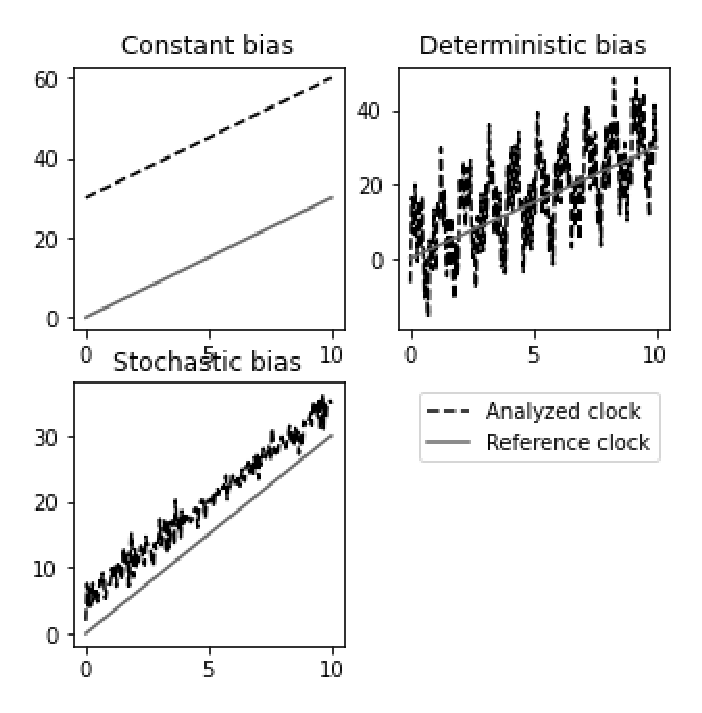
\includegraphics[width=0.5\textwidth]{figures/bias_examples}
	\caption{Example of clock readouts depending of nature of their bias}
\end{figure}
More information on exact clock and noise models will be given in following sections.

%----------------------------------------------------------------------------------------------------
\subsection{Basic clock model}
Basic clock model is a deterministic representation of clock as a second-order linear differential
equation.
\begin{equation}
	\label{equ:basic_clock}
	\ddot{x}(t)=z(t).
\end{equation}
Solution to that equation is
\begin{equation}
	\label{equ:basic_clock_solved}
	x(t)=x_{0}+y_{0}\tau+0.5z_{0}\tau^{2},
\end{equation}
where:
\begin{itemize}
	\item $x(t)$ is clock measurement at time $t$, also called time-offset or bias,
	\item $y(t)$ is fractional frequency offset,
	\item $z(t)$ is fractional frequency drift,
	\item $\tau$ is time difference defined as $\tau = t-t_{0}$.
\end{itemize}
Values $x_{0}$, $y_{0}$, $z_{0}$ refer to initial state of model at $t=t_{0}$.
Because frequency stability of clock degrades over time, as a result of ageing of physical 
components that they consist of, fractional frequency drift is sometimes called clock 
ageing parameter.
In this work $z(t)$ will be also referred to as the linear frequency drift. This terminology
was applied as in case of data used in this research there is a observable deterministic 
first order frequency drift behaviour.

%----------------------------------------------------------------------------------------------------
\subsection{Oscillator noise model}
Basic clock model is limited as it allows only for description of simple deterministic systems 
while real life implementations of clock are complex system with both deterministic and 
stochastic components. 
As described in section \ref{sec:physical_clock} of this chapter central element of every clock,
including atomic clocks, is an oscillator. That is why to create a more complex clock models 
an oscillator noise model must be created.
Role of this model is to derive a clock frequency and phase form an actual physical observation 
which in case of an atomic clock is voltage signal.
Equation describing voltage level on quartz oscillator, which is type of oscillator present in
atomic clocks, can be described by an equation:
\begin{equation}
	\label{equ:quartz_voltage}
	U(t)=(U_{0}+\epsilon(t))sin(2\pi \nu_{0}t + \phi(t)),
\end{equation}
where:
\begin{itemize}
	\item $U_{0}$ is peak voltage amplitude,
	\item $\nu_{0}$ is nominal frequency,
	\item $\phi(t)$ represents random phase deviations,
	\item $\epsilon(t)$ represents random amplitude deviations.
\end{itemize}
Since variation in signal amplitude do not influence measurements of signal frequency, save for
extreme cases where it drops so low that signal peak is not registered, it can be ignored in 
equation used for frequency stability analysis.
This means that equation actually used is:
\begin{equation}
	\label{equ:quartz_voltage_simplified}
	U(t)=U_{0}sin(2\pi \nu_{0}t + \phi(t)).
\end{equation}
Instantaneous clock frequency can be defined as the time derivative of the phase as demonstrated
on following equation:
\begin{equation}
	\label{equ:inst_frequency}
	\nu(t) = \nu_{0}+ \frac{1}{2\pi} \frac{d\phi}{dt},
\end{equation}
where $\frac{d\phi}{dt}$ represents instantaneous frequency offset.
The performance of the clock oscillator is determined by the frequency stability and not 
total frequency and the value of frequency offset is usually small in relation to measured.
Because of that it is more meaningful to describe clock stability with normalized, or fractional,
frequency as described in equation:
\begin{equation}
	\label{equ:normalized_frequency}
	y(t) = \frac{\nu(t)-\nu_{0}}{\nu_{0}} = \frac{dx}{dt}
\end{equation}
where
\begin{equation}
	\label{equ:what_is_time_offset}
	x(t) = \frac{\phi(t)}{2\pi \nu_{0}}
\end{equation}
is bias described in the units of time.


%----------------------------------------------------------------------------------------------------
\subsection{Standard clock model}
Standard clock model is most commonly used mathematical description of the clock that models it as
driven by an oscillator that is in periodic motion around a nominal frequency.
It models how precise clocks are subject to both deterministic bias as well as stochastic 
frequency fluctuations.
Mathematically the standard clock model is represented as a first order stochastic differential
equation . Two state model, with states representing time offset and fractional frequency offset
is described by Galleani. However in this work more focus will be given to three state model 
with states representing clock bias, fractional frequency offset and frequency drift.
This model was presented by Chaffee in 1987 and is described as :
\begin{equation}
	\label{equ:three_state_clock}
	\left[ \begin{array}{c} dx(t)\\ dy(t)\\ dz(t) \end{array} \right] =
	\left[ \begin{array}{ccc} 0& 1& 0\\ 0& 0& 1\\ 0& 0& 0 \end{array} \right]
	\left[ \begin{array}{c} x(t)\\ y(t)\\ z(t) \end{array} \right] dt +
	\left[ \begin{array}{c} d\epsilon(t)\\ d\zeta(t)\\ d\eta(t) \end{array} \right] 
\end{equation}
which is using matrix notation can be described as :
\begin{equation}
	\label{equ:clock_matrix}
	dX(t) = AX(t) +dB(t).
\end{equation}
In those equations $x(t)$, $y(t)$ and $z(t)$ are respectively clock bias, fractional frequency and
fractional frequency drift while $\epsilon(t)$ $\zeta(t)$ and $\eta(t)$ are zero mean Gaussian
white noise processes. They are described as:
\begin{itemize}
	\item $\epsilon(t)$ is white frequency modulation (WFM),
	\item $\zeta(t)$ is random walk frequency modulation (RWFM),
	\item $\eta(t)$ is random run frequency modulation (RRFM).
\end{itemize}
With this it is clear that in matrix notation $X$ is clock state matrix, $A$ is state transition
matrix while $B$ is random noise matrix.
As this work do not focuses on stochastic differential equations only a solution for the equation
\ref{equ:three_state_clock} will be shown, for those more interested in how it was calculated 
more basic literature on topic of SDE is suggested.
\begin{equation}
	\label{equ:clock_solved}
	X(t) = \Phi(t,t_{0})X(t_{0}) + \int^{t}_{t_0}\Phi(t,\tau)dB(\tau),
\end{equation}
where
\begin{equation}
	\label{equ:what_is_phi}
	\Phi(t,t_{0}) = e^{At-t_{0}} = \sum^{\infty}_{0}\frac{(A(t-t_{0}))^2}{n!},
\end{equation}
and $X_{0}$ is the initial condition.
If $X(t_{0})$ is assumed to be a non-random constant then $X(t)$ is a Gaussian process with 
stationary increments and clock bias at time $t$ can be calculated with equation:
\begin{equation}
	\label{equ:bias_final}
	x(t)=x(t_{0}) + y(t-t_{0}) + z(t_{0})\frac{(t-t_{0})^2}{2} + \int^{t}_{t_{0}}d\epsilon(\lambda)
	+ \int^{t}_{t_{0}}(t-\lambda)d\zeta(\lambda) 
	+ \int^{t}_{t_{0}}\frac{(t-\lambda)^2}{2}d\eta(\lambda),
\end{equation}
where the integrals represent noise processes and terms above 2 are excluded.

%====================================================================================================
\section{Stability analysis}
Quality of an oscillator is determined by its frequency stability over time. 
As both phase and frequency influence clock readouts so stability analysis must focus on both.


%----------------------------------------------------------------------------------------------------
\subsection{Allan variance}
Allan variance, also know as the two-sample variance, is the default descriptive statistic
for time and frequency measurements.
This is because standard variance is not suitable for modelling non stationary processes.
The Allan variance is formally adopted as a standard for characterising and reporting instabilities
in phase, frequency or amplitude measurements in time domain.
Allan variance is an infinite time average of the square of the difference of two fractional
frequency measurements:
\begin{equation}
	\label{equ:allan_first}
	\sigma^{2}_{y}(\tau)=0.5\langle (\hat{y}_{k+1}-\hat{y}_k)^{2}  \rangle,
\end{equation}
where $\langle \rangle$ denotes the infinite time average operator while $\hat{y}_k$ is a 
frequency at time $t_{k}$. Hat over variable indicates that value is estimated from phase
measurements with following equation:
\begin{equation}
	\label{equ:y_hat}
	\hat{y}_{k}=\frac{1}{\tau}\int^{t_{k+1}}_{t_{k}}y(t)dt =
	\frac{x(t_{k+1})-x(t_{k})}{\tau},
\end{equation}
In real world application Allan variance is calculated basing on the set of a measurements which
is always a finite set. Therefore as data worked upon is finite and discrete in time domain 
Allan variance can be described as:
\begin{equation}
	\label{equ:allan_discrete}
	\sigma^{2}_{y}(\tau) = \frac{1}{2(M-1)}\sum^{M-1}_{k=1}(\hat{y}_{k+1}-\hat{y}_{k})^2,
\end{equation}
where $M$ denotes number of measurements.
By substituting selected values in equation \ref{equ:allan_discrete} Allan variance can be
described as a function of phase or time offset
\begin{equation}
	\label{equ:allan_discrete2}
	\sigma^{2}_{y}(\tau) = \frac{1}{2(M-1)\tau^{2}}\sum^{M-1}_{k=1}(x_{k+2}-2x_{k+1}+x_{k})^2.
\end{equation}
Even better estimation of Allan variance can be achieved by calculating what it is called a
overlapping Allan variance. This is because it forms all possible overlapping combinations of
available data
\begin{equation}
	\label{equ:overlapping_allan}
	\sigma^{2}_{y}(\tau) = \frac{1}{2(N-2m)\tau^{2}}\sum^{N-2m}_{k=1}(x_{k+2m}+2x_{k+m}+x_{k})^2.
\end{equation}
As overlapping Allan variance provides better results than its basic version in most cases 
literature dealing with stability analysis will use term Allan variance to refer to it 
overlapping version unless specified otherwise.
There is also one more variant called modified Allan variance that unlike all previous examples
can distinguish between WPM and FPM.
In term of phase modified Allan variance is described as:
\begin{equation}
	\label{equ:modified_allan}
	\sigma^{2}_{y}(\tau)=\frac{1}{2m^{2}\tau^{2}(N-3m+1)\tau^{2}}\sum^{N-3m+1}_{j=1}(
	\sum^{j+m-1}_{k=j}(x_{k+2m}-3x_{k+m}+x_{k})^2)
\end{equation}

%--------------------------------------------------------------------------------------------------
\subsection{Hadamard variance}
Hadamard variance was derived from the Hadamard transform for use in stability analysis by 
Baugh.  As the Allan variance describes a second-order phase variation so Hadamard variance 
describes third-order phase variation.
Unlike Allan variance Hadamard variance is insensitive to linear frequency drift, this is 
especially important in context of this work as rubidium clocks used in GPS satellites have a 
prominent linear drift.
As with Allan variance the overlapping version of equation is used as default:
\begin{equation}
	\label{equ:overlapping_hadamard}
	\sigma^{2}_{H} = \frac{1}{6(N-3m)\tau^2}
	\sum^{N-3m}_{k=1}(x_{k+3m}-3x_{k+2m}+3x_{k+m}-x+{k})^{2}
\end{equation}

%====================================================================================================
\section{Modeling noise}
Noise process is defined as a stochastic time varying phenomenon that at each moment in time is
represented by a random variable $X(t)$ whose probability density function is denoted as $f_{X}(t)$.
Such process can be either continuous or discrete depending on model that is worked on, in case 
of real life application $f_{X}(t)$ may not be known.
In context of time and frequency metrology such signal components are modelled as a power-law
noise processes. This is special type of noise process whose frequency and phase noise power 
spectral densities vary as as a power of the Fourier frequency.
Power noise process can be described in relation to frequency fluctuations as:
\begin{equation}
	\label{equ:power_noise_freq}
	S_{y}(f) \propto f^{\alpha},
\end{equation}
where $S_{y}(f)$ denotes fluctuations of frequency $f$ and $\alpha$ describes a power-law of
frequency noise.
When dealing with time measurements it can be more useful to describe a relation between clock 
bias, also called a phase variation, and noise:
\begin{equation}
	\label{equ:power_noise_phase}
	S_{x}(f)=\frac{S_{y}(f)}{(2\pi f)^2} \propto f^{\beta},
\end{equation}
where $\beta$ is description of power-law phase noise and is calculated as $\beta=\alpha-2$.
Power-law noise can also be described in time domain in relation to Allan variance.
In this form process is described as :
\begin{equation}
	\label{equ:power_noise_time}
	\sigma^{2}_{y}(\tau)=g_{\gamma}\tau^{\gamma}
\end{equation}

----------------------------------------------------------------------------------------------------
\subsection{Oscillator noise as linear combination of power-law noises}
In general there are five distinct power-law processes, white phase modulation (WPM), flicker 
phase modulation (FPM), white frequency modulation (WFM), flicker frequency modulation (FFM) and
random walk frequency modulation (RWFM).
All of them can be described by parameters $\alpha$, $\beta$, $\gamma$
\begin{table}[htb] 
	\centering
	\caption{Parameters of power-law noise variants}
	\label{tab:power-noise}
	\begin{tabular}{lccc}
		\hline
		\hline
		Noise type& $\alpha$& $\beta$& $\gamma$\\
		\hline
		WPM&   2 &  0& -3\\
		FPM&   1 & -1& -2\\
		WFM&   0 & -2& -1\\
		FFM&  -1 & -3& -0\\
		RWFM& -2 & -4&  1\\
		\hline
		\hline
	\end{tabular}
\end{table}
The power spectral density of oscillator noise is described as a linear combination of 
those power noise processes:
\begin{equation}
	\label{equ:linear_noise_comb}
	S_{y} = \sum_{\alpha=-2}^{2}h_{\alpha}f^{\alpha},
\end{equation}
where $h_{\alpha}$ indicates influence of a specific noise type on overall oscillator noise.
For general time representation a modified Allan variance can be used:
\begin{equation}
	\label{equ:allan_noise_comb}
	\sigma^{2}_{y} = \sum_{\gamma=-3}^{1}g_{\gamma}\tau^{\gamma},
\end{equation}
where $\tau$ is analysis interval.
%----------------------------------------------------------------------------------------------------
\subsection{White phase modulation noise}
White phase modulation noise is a constant-mean, constant-variance stochastic process.
Discrete white phase modulation noise is represented by a sequence of independent random variables
with identical Gaussian probability density functions which are denoted as  
$\mathcal{N}(\mu,\sigma^{2})$
\begin{figure}[htb] 
	\label{fig:wpm}
	\centering
	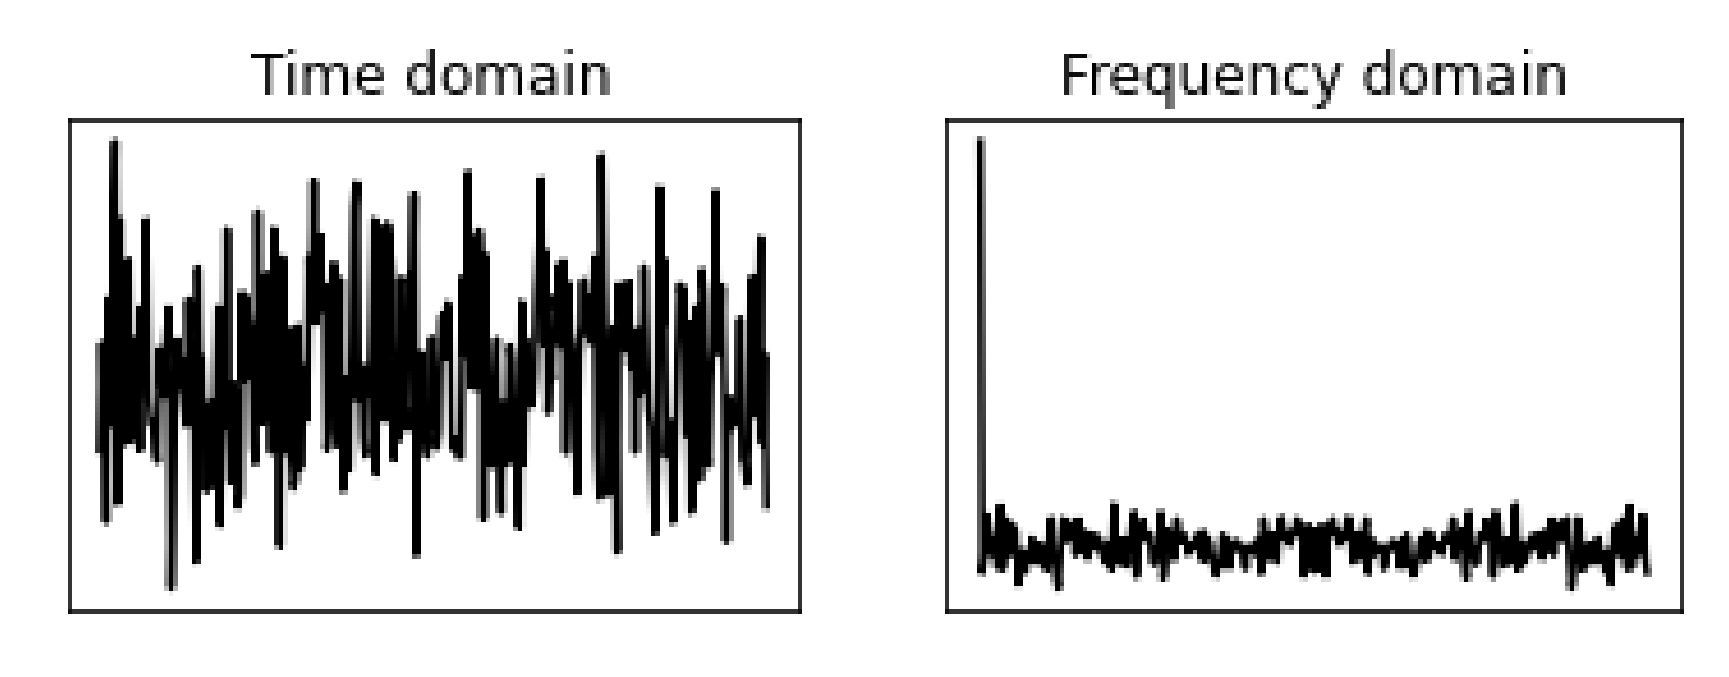
\includegraphics[width=0.7\textwidth]{figures/wpm}
	\caption{White phase modulation in time and frequency domains}
\end{figure}

%----------------------------------------------------------------------------------------------------
\subsection{Flicker phase modulation noise}


%----------------------------------------------------------------------------------------------------
\subsection{White frequency modulation noise}
White frequency modulation is a zero mean white noise sequence 

%----------------------------------------------------------------------------------------------------
\subsection{Flicker frequency modulation noise}

%----------------------------------------------------------------------------------------------------
\subsection{Random walk frequency modulation noise}




%====================================================================================================
\section{State of the art in GPS clock bias prediction}

%----------------------------------------------------------------------------------------------------
\subsection{Time references in GPS}
For correct implementation of beacon based navigation a spatial and temporal reference frames 
must be agreed upon. In case of GPS information about it can be found in International Earth
Orientation Service Conventions. Due to the scope of this work attention will be given only to
standards related to time measurements. The first temporal reference that have to be introduced
is Geocentric Coordinated Time (TCG). It is a timescale that is defined to be consistent with
general relativity theory in proximity of the non-rotating Earth. Due to that TCG can not be
directly observed an as such is used only as a theoretical standard of timescale.
Next step is definition of still theoretical but physically realizable Terrestrial Time (TT).
Relation between TCG and TT is described as:
\begin{equation}
	\label{equ:tcg_to_tt}
	\frac{dTT}{dTCG} = 1 - \frac{W_{0}}{c^2},
\end{equation}
where $W_{0} = 62636857 m^{2}/s^{2}$ is the Earths gravitational potential at sea level.
This theoretical concept is realised as the International Atomic Time (TAI) which is an
atomic timescale relying on ensemble of frequency sources placed at multiple locations around 
the globe. Base of time measurement for TAI is the SI second which is defined as 
\textit{
	duration of 9 192 631 770 periods of the radiation corresponding to the transition between
	two hyperfine levels of the ground state of the cesium 133 atom, with the cesium atom at 
	rest on the rotating geoid at a temperature of 0 K.
}
TAI is used as a frequency standard for Coordinated Universal Time (UTC) which is the most
commonly used time reference frame in civilian purposes.
In case of GNSS applications TAI is not accessible in real time, therefore a realisation of 
TT dedicated to GNSS must be realised.
For GPS, the World Geodetic System 1984 (WGS84) is adopted with relevant timescales being 
GPS System Time (GPST) ant the realisation of UTC at the United States Naval Observatory 
(UTC(USNO)). GPST is the reference timescale for all GPS devices, both satellites and ground
recievers. Main difference between GPST and UTC is that GPST is a continuous timescale while 
UTC introduces concept of leap seconds.
Relationship between GPST and TAI can be described as:
\begin{equation}
	\label{equ:gpst_to_tai}
	T_{TAI}-T_{GPST} = 19 + X_{USNO},
\end{equation}
where $X_{USNO}$ is bias of US Naval Observatory clock in relation to TAI such that 
$|X_{USNO}| \le 1\mu s$. Value of $19$ seconds is added as zero epoch of GPST is set on 
6 January 1980 and is 19 seconds ahead of TAI zero epoch.

%----------------------------------------------------------------------------------------------------
\subsection{Satellite broadcast polynomial}

%----------------------------------------------------------------------------------------------------
\subsection{IGU products}
The most widely used source of precise clock corrections are products provided 
by International GNSS Service (IGS) \cite{Kouba2009}.
\begin{table}[htb] 
	\centering
	\caption{Variants of IGS products}
	\label{tab:igs_products}
	\begin{tabular*}{\textwidth}{*{5}{l}}
		\hline
		\hline
		Type& Accuracy& Latency& Update& Sample \\
		&&&&interval\\
		\hline
		Broadcaster & 5ns & real time & -- & daily  \\
		Ultra rapid -- predicted & 3ns & real time & at 03, 09, 15, 21 UTC & 15 min  \\
		Ultra rapid -- observed & 150ps & 3-9 hours & at 03, 09, 15, 21 UTC & 15 min  \\
		Rapid & 75ps & 17-41 hours & at 17 UTC daily & 5 min \\
		Final & 75ps & 12-18 days & every Thursday & 30 s \\
		\hline
		\hline
	\end{tabular*}
\end{table}
Values shown in Table \ref{tab:igs_products} refer to satellite clock bias only,  IGS products
provide other information which full description  is available at online repository. 
IGS products can be easily divided into two categories:
\begin{itemize}
	\item real time consisting of transmitted and ultra rapid predicted half,
	\item high latency consisting of ultra rapid observed half as well as rapid and final products.
\end{itemize}
Solutions that have high latency are not usable in real-time navigation and as such will not be
considered in this work. Ultra-rapid observed will be used as a source of
reference time so that if a bias prediction error is equal to zero it means that is
the same as provided by ultra-rapid observed.
As can be seen in Table \ref{tab:igs_products} all real-time solutions provide precision 
at a range of nanoseconds, aim of this work is to show that LSTM networks can provide 
better results than those solutions while still working at real-time response latency.

This work focuses only on GPS satellites which are divided into following blocks:
I, II, IIA, IIR ,IIR-M ,IIF, III.
Blocks I and II were fully retired before research described in that paper began and block
III satellites were active for to short time to generate enough data.
That is why those blocks were not used at all, on the other hand single satellite from block
IIA was used in second phase of experiments however it was retired in mean time and a decision
was made to not use it in next experiments and as such it is not listed in final satellite pool.
This results in total of 30 satellite clocks analyzed with almost all of them are equipped 
with Rubidium clock ensemble witch exception of two satellites from generation IIF 
that use Cesium clocks instead.
Each satellite have an assigned space vehicle number (SVN) and pseudo random noise (PRN).
In this work a PRN will be used as a identifier as it is unique for every active satellite, 
although it can be used again after said satellite gets retired, and ranges from 1 to 32.
Association between satellite PRN, clock and block is shown in Table \ref{table:prn}
\begin{table}[htb] \label{table:prn}
\parindent0pt
\caption{Bias prediction error in relation to regularization and dropout level}
\centering
\begin{tabular}{ l  c  c }
  \hline
  \hline
  Generation& clock type& satellites\\  \hline
  IIA & Rb& 18\\  
  IIR & Rb& 2 11 13 14 16 19 20 21 22 23 28\\ 
  IIR-M & Rb& 5 7 12 15 17 29\\ 
  IIF & Rb& 1 3 6 9 10 25 26 27 30 32\\ 
  IIF & Cs& 8 24 \\ \hline \hline
 \end{tabular}
\end{table}
For satellites with rubidium based clock ensembles bias have a very distinct constant drift
that makes data appear linear, it can be seen for satellites 01 and 08. 
On the other hand in case of cesium based clock ensembles for which constant drift is much 
smaller other sources of bias are visible, like seen for satellite 24.
There is also a single satellite for which, during observed period, constant drift was almost
not present. This was satellite 14 and while no official source of information describes this 
behaviour


\chapter{Machine learning based approach}


%====================================================================================================
\section{Concepts in machine learning}

%----------------------------------------------------------------------------------------------------
\subsection{Differences between knowlege and data based models}

%----------------------------------------------------------------------------------------------------
\subsection{What is a machine learning algorithm}

%----------------------------------------------------------------------------------------------------
\subsection{Deep learning}

%====================================================================================================
\section{Non neuron approaches}

%----------------------------------------------------------------------------------------------------
\subsection{Basics of regression}

%----------------------------------------------------------------------------------------------------
\subsection{Gradient approach}

%----------------------------------------------------------------------------------------------------
\subsection{Polynomial regression}

%----------------------------------------------------------------------------------------------------
\subsection{Gradient based adjustment}

%----------------------------------------------------------------------------------------------------
\subsection{Support vector machine}


%====================================================================================================
\section{Neural networks}

%----------------------------------------------------------------------------------------------------
\subsection{Feed forward neural networks}

%----------------------------------------------------------------------------------------------------
\subsection{Simple reccurent neural networks}

%----------------------------------------------------------------------------------------------------
\subsection{Networks with long term memory}


\chapter{Neural networks}


%====================================================================================================
\section{History}

%----------------------------------------------------------------------------------------------------
\subsection{Biological inspiration}
Artificial neural networks were originaly created as a way of modeling behavior of biological
neurons.
Neurons are at their core cells so most of metabolic processes common for animal cells also
occur in them. However just like red blood cells neural cells do not divide on their own and new
neurons are generated by specialised stem cells.
\begin{figure}[hb]
	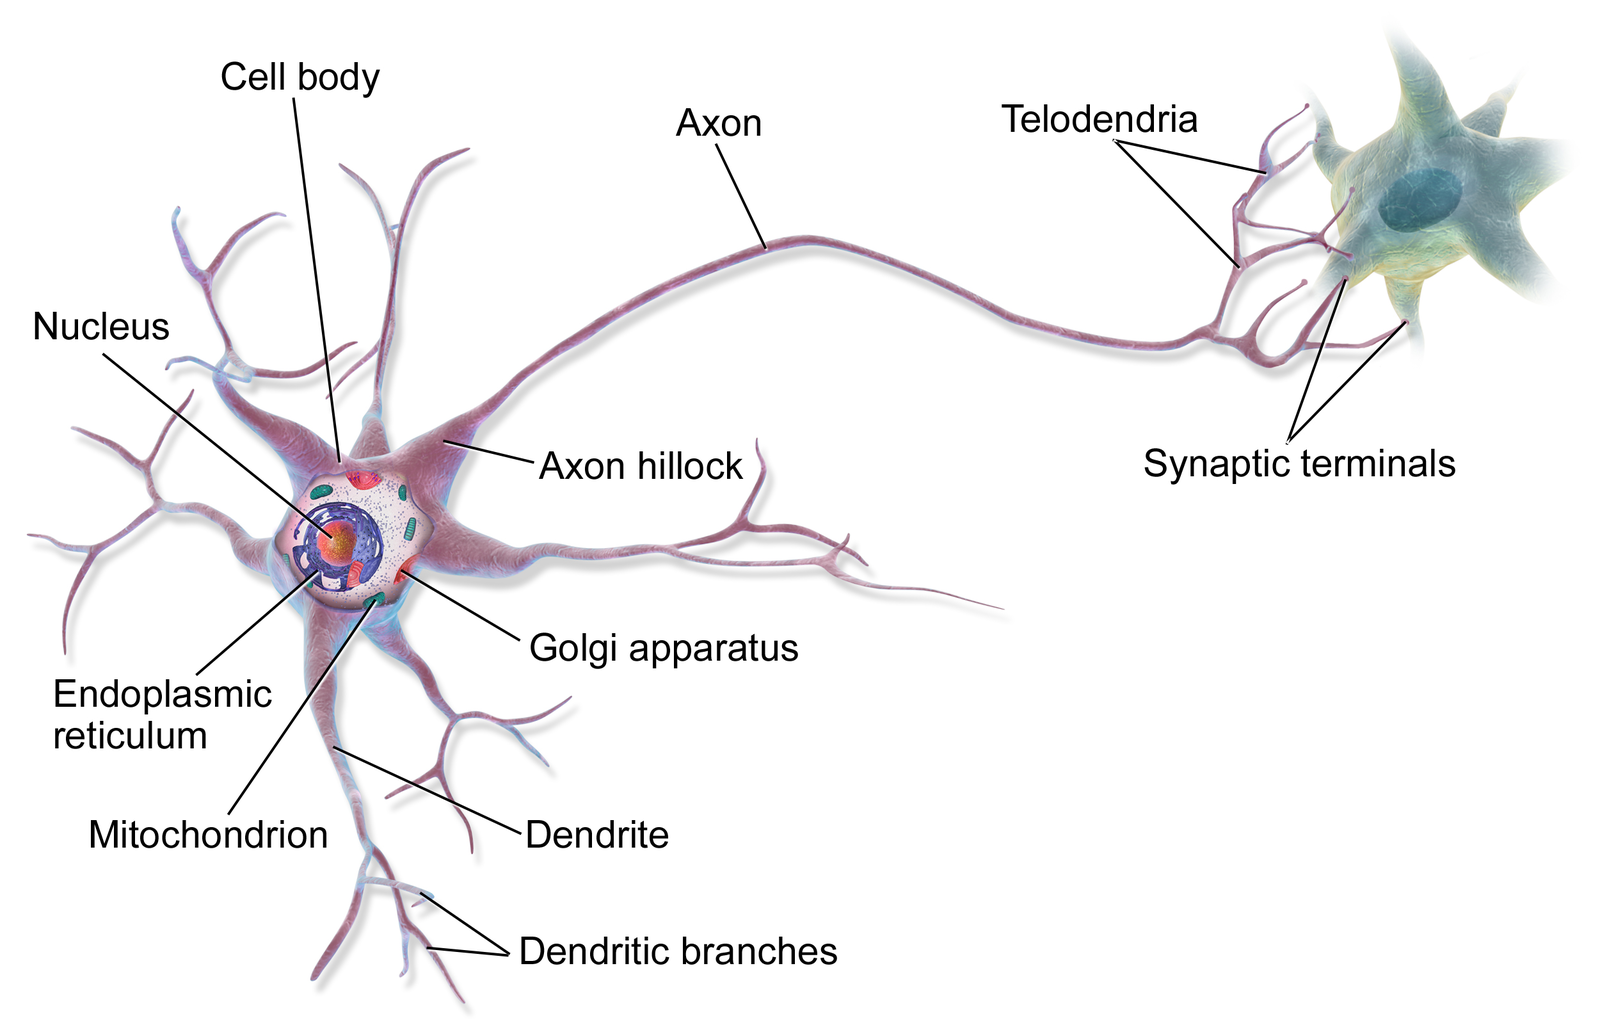
\includegraphics[width=\textwidth]{res/Blausen_MultipolarNeuron}
	\caption{Neural cell structure. Image by Bruce Blaus}
	\label{fig:Blausen-Neuron}
\end{figure}
There is however one behavior that until recently was believed to be specific to only neural cells
and even recent studies extend this ability to glial cells only.
This is ability to transfer a electric signal trough length of cell axon 

%----------------------------------------------------------------------------------------------------
\subsection{Cybernetics, first steps in modeling of neural systems}
The first branch of science that tried do decopule neuron models from its biological basis was 
cybernetics. The term cybernetics originates from greek word \textbf{TODO: GREEK LETTERS} which
originally meant a helmsman. However even Aristotel used it to describe people that control 
other systems then boat. In modern Greek KIBRNETES means either a manager or a control system and 
helmsman is called PEDALIONHOS.
Term cybernetics was first used in its moder meaning by Norbert Wiener in 1948 in book 
``Cybernetics or control and Communication in the Animal and the Machine''. 
In that publication Wiener describes application of technical and mathematical analysis 
that was used for mechanic systems to biological organisms.
\begin{figure}[hb]
	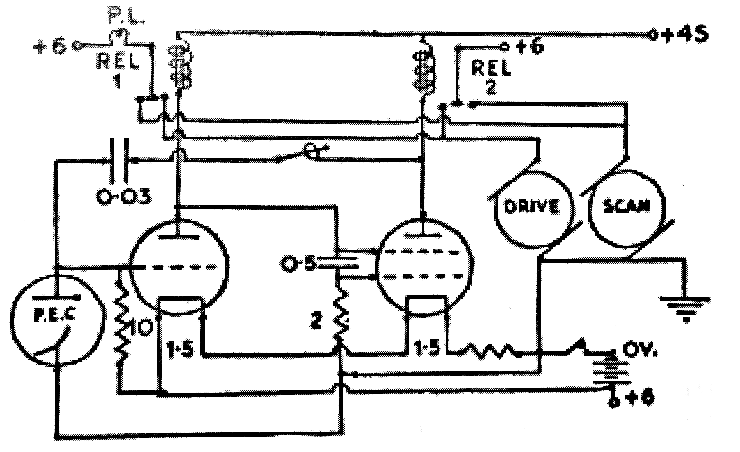
\includegraphics[width=\textwidth]{res/speculatrix}
	\caption{Machina speculatrix}
	\label{fig:machina_speculatrix}
\end{figure}




%====================================================================================================
\section{Feed forward neural networks}

%----------------------------------------------------------------------------------------------------
\subsection{Mathematical model of neuron}
First mathematical model of the neural cell was created in 1943 by Warren MuCulloch and Walter Pitts.
It aimed at recreating an behavior of the neuron electric potenitial activation as a result of
synaptic potential reaching specific bias. What is important this model was never supposed to
precisely mimic behavior of biological neuron and as such do not include representation of metabolic
processes or even neurotransmition.
However despite significant simplification McCulloch-Pitts neuron proven to have many uses and
its basic structure were used to create most of modern day models.
Essentialy in this model neuron is a finction $f_n(x):\mathbb{R} \rightarrow \{ 0,1 \} $ where $n$
is size of input.
In such case equation describing neuron response is as follows:
The basic model of the neuron (neural layer) was created in 1943 by McCullough and Pitts 
\cite{McCulloch1943}. It described response of neural layer to multiple signals with
equation $y= \chi (W\cdot x+b)$, where $y$ is response, $x$ input, $W$ weights, $b$ bias and
$\chi$ is a step function.
Algorithm for automated adjustment of weights in relation to data was proposed in 1958
by Rosenblatt \cite{Rosenblatt58}. This model and all its successors can be described
as an aggregation, dampening, and activation signal path.
\begin{figure}[h] 
	\centering
	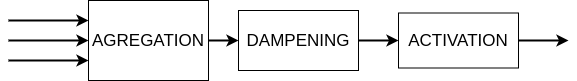
\includegraphics[width=10cm]{res/basic_neuron}
	\caption{Generalized model of a neuron}
	\label{fig:basic_neuron}
\end{figure}
In the case of McCullough-Pitts neuron aggregation is a weighted sum, dampening is the subtraction
of a bias and activation is a step function. While other models have some differences,
usually different activation functions, the basic signal flow remains unchanged.
While this model and its successors were inspired by a biological neuron there are much
more simplified. One of those simplifications is the lack of time-domain in the model which means
that response of a layer depends only on its current input.
This is in contrast with biological networks that are sensitive not only for a signal value
but also for its change over time.

%----------------------------------------------------------------------------------------------------
\subsection{Perceptron, abilities and limitations}
Simple perceptron is a McCullouch-Pitts neuron with a learnig alorithm assigned to it.
Therfore perceptron equation can be described as a :
\begin{equation}
	y = \chi (W\cdot x+b),
\end{equation}
where $\chi$ is a step function described as:
\begin{equation}
	\chi (x) =  
	\begin{cases}
		1        \quad \text{if } u > 0\\
		0        \quad \text{if } u \leq \\
	\end{cases}
\end{equation}
As perceptron rule is an example of a supervised learning it reqire a training set where for 
each input $x_{j}$ a corresponding expected output $d_{j}$ is provided. 
Then algorithm adjusts weights and bias of given neuron so that it response will 
correspond to expected one. 
Weights and biasa together are considered parameters of neuron and described as a:
\begin{equation}
	\phi = \{ W,b \}.
\end{equation}
\textbf{TODO: ADD A NEURON DIAGRAM}
Percetron rules works by excuting following steps:
\begin{itemize}
	\item If value of $y_{j}$ is equal to expected value $d_{j}$ then weights $W$ and 
		  bias $b$ remain unmodified.
	\item If value $y_{j}=0$ and $d_{j}=1$ then weights are to be updated acording to 
		  equation $W:=W+x_{j}$ and bias acording to equation $b:=b+1$.
	\item If value $y_{j}=1$ and $d_{j}=0$ then weights are to be updated acording to 
		  equation $W:=W-x_{j}$ and bias acording to equation $b:=b-1$.
\end{itemize}
After parameter update a new input-output pair is presented and algorithm repeats until all 
pairs from learning set are processed.
Perceptron rule was later generalied into a Widrow-Hoff rule according to which parameters are 
updated as described in equation :
\begin{equation}
	\Delta W_{j} = x_{j}(d_{j}-y_{j}),\\
	\Delta b_{j} = d_{j} - y_{j},\\
	W :=  W + \Delta W_{j},\\
	b := b + \Delta b_{j}.
\end{equation}
If only possible responses of neuron are 0 and 1 then Widrow-Hoff rule behaves exactly like a
perceptron rule.
Aim of lerning is minimalization of energy function of neuron response which is described as a:
\begin{equation}
	E = \sum_{j=0}^{n}(y_{j}-d_{j})^{2}
\end{equation}
Because step function is not continous in point 0 it is impossible to calculate it derivative
an therfore gradient based learing algorithms cannot be used for perceptron.
This limits this model to a single layer nework which is hightly problematic as such network
is very limited in its applications.
One of most basic examples ccan be a inability of perceptron to realize XOR function.
This is because in case of two dimensional input perceptron divides space into two lineary
seperable subspaces.
\begin{figure}[h] 
	\centering
	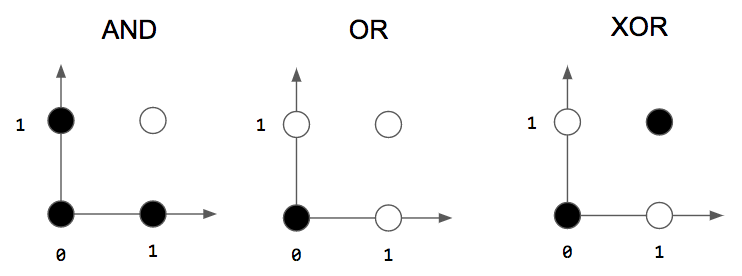
\includegraphics[width=10cm]{res/logic_neuron}
	\caption{Logic functions presented on 2D space}
	\label{fig:logic_neuron}
\end{figure}
Exculsive alternative do to its nature is not a lineary seperable function. It is however
possible to create a realization of XOR with perceptron like neurons by recreating a logic
circuit that is equivalent to XOR while using only OR, NOT, AND gates.
\begin{figure}[ht] 
	\centering
	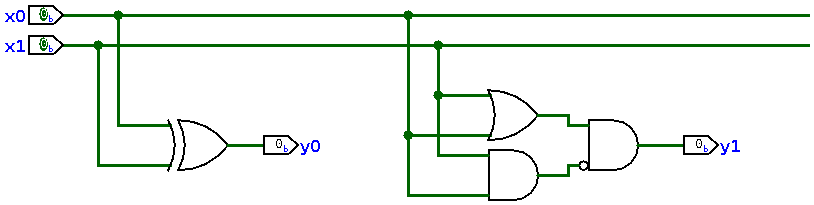
\includegraphics[width=\textwidth]{res/xor_circ}
	\caption{XOR circuit and it equivalent}
	\label{fig:xor_circ}
\end{figure}
However while such network will process data it cannot learn anything new, to solve that 
problem a new approach must be taken.

%----------------------------------------------------------------------------------------------------
\subsection{Backpropagation and multi layer neural networks}
First succesfull atempt at creating learning algorithm for multilayer neural network was made
in 1986 year by Rumelhart, Hinton and Williams. That algorithm was a backpropagation and as it
requires calcualation of simple gradient underlying activation function must be differentiable.
Because of that step function was repleaced bya logistic function as the neuron activation.
There is a unipolar variant
\begin{equation}
	f_{a}(u) = \sigma(u) = \frac{1}{1+e^{-\beta u}},
\end{equation}
which alongside its bipolar eqiuvalent
\begin{equation}
	f_{a}(u)=tanh(\beta u),
\end{equation}
became most widely used activation functions.
\textbf{TODO:ADD PLOTS FOR VARIOUS BETA VALUES}
Important trait of sigmoidal function is it differenciability. In case of unipolar function
with $\beta = 1$ resulting \textbf{TODO: JAK JEST ROZNICZKA PO ANGIELSKU} is described as a 
\begin{equation}
	\frac{df_{a}(u)}{du}=f_{a}(u)(1-f_{a}(u)).
\end{equation}
In case of bipolar function with $\beta = 1$ result is as follows:
\begin{equation}
	\frac{df_{a}(u)}{du}=1-f_{a}^{2}(u).
\end{equation}
Those functions are trivial to calculate nuerically as all they require is value of a base
function for given input. It is also worth noting that for $\beta \rightarrow \inf$ sigmoidal
functions start to behave like a step function.
Backpropagation is an example of supervised learning where a energy function of te neuron
response is minimmized
\begin{equation}
	E=\frac{(y-d)^{2}}{2}
\end{equation}
With that we can calculate a gradient for a j-th input, desired output pair with an following
equation:
\begin{equation}
	\Delta_{j}E = \frac{\partial E}{\partial W_{j}} = (y_{j}-d_{j})x_{j}\frac{df_{a}(u_{j})}{du_{j}}. 
\end{equation}
For conviniece it is reasonable to write a part related to neuron response as a:
\begin{equation}
	\delta_{j} = (y_{j}-d_{j})\frac{df_{a}(u_{j})}{du_{j}}, 
\end{equation}
so that discreete weight update function can be written as a 
\begin{equation}
	W := W - \eta \delta_{j} x_{j},
\end{equation}
where $x_{j}$ is related to network input,  $\delta_{j}$ to output and $\eta \in <0,1>$ is a 
constant learning factor.
Learning factor is considered a metaparameter and is set once for whole learning process, 
therfore a seto of metaparameters for simple backporbagation algortihm can be described as 
a $\Phi = \{\eta \}$. There is also a continous approach to adjusting network parameters that
relies on solving differencial equation
\begin{equation}
	\frac{dW_{j}}{dt} = -\mu \delta_{j} x_{j},
\end{equation}
where $\mu$ is equivalent of $\eta$ from discrete model. However as this work focuses on 
numerical solutions a discrete model was chosen and no more attention will be given to a 
continous one.
Choice of correct learning rate is crucial in designing a efficen backpropagation 
learning algorithm as two small value can result in slow convergence rate and high risk of 
getting stuck in local minima. On the other hand high learning rate may result in algorithm
jumping over desired solution and never converging on it. 
\begin{figure}[ht] 
	\centering
	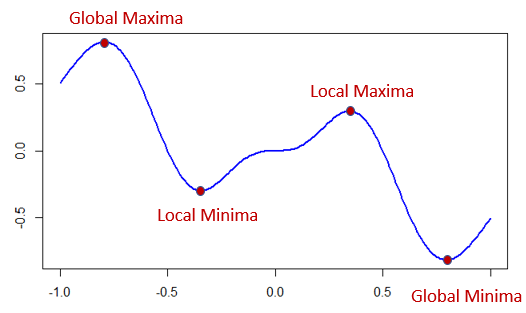
\includegraphics[width=\textwidth]{res/local_minima}
	\caption{Example of local and global minima}
	\label{fig:local_minima}
\end{figure}

%----------------------------------------------------------------------------------------------------
\subsection{Other gradient based optimalizators}
\subsubsection{Momentum}
\subsubsection{Nesterov}
\subsubsection{AdaGrad}
\subsubsection{RMSProp}
\subsubsection{Adam}

%----------------------------------------------------------------------------------------------------
\subsection{Limitations on neural networks depth}


%====================================================================================================
\section{Recurrent networks and deep learning}

%----------------------------------------------------------------------------------------------------
\subsection{Deep learning models}

%----------------------------------------------------------------------------------------------------
\subsection{Simple recurrent networks}
Simple solution to problem of time independence is to concatenate response of neural layer
from previous cycle to it input $x'(t)=[x(t)|y(t-1)]$.
Such solution results in signal propagating trough time and influencing responses of future cycles,
if this is the only modification to the feed-forward model such layer is called Simple Recurrent
Unit (SRU).
\begin{figure}[h] 
	\centering
	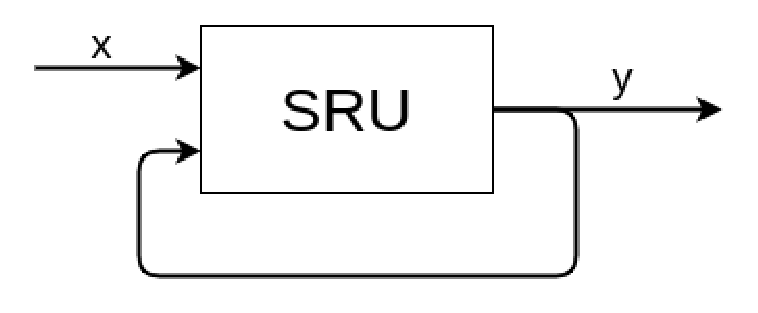
\includegraphics[width=5cm]{res/sru}
	\caption{Simple Reccurent Unit (SRU)}
	\label{fig:sru}
\end{figure}
While this solution makes model time aware it has its own problems, mainly a signal vanishing
issue. Since the input signal from a cycle, $n$ has direct influence only on a response of this
cycle and for each subsequent cycle, it is the only through a feedback loop.
Influence of input $n$ on response of cycle $n+k$ grows inverse proportional to $k$.
This means that in this model only those regularities that appear over short time periods can
be detected.
Making weights on feedback bigger will not eliminate the problem and instead replace it with signal
an explosion that causes a response to reach maximum value if a strong signal appeared on input at
least once.

%----------------------------------------------------------------------------------------------------
\subsection{Long short term memory networks}
One of the possible solutions to this issue is the addition of long term memory which will regulate
forward and loopback path influence on neuron response, such a solution is used in long short
term memory (LSTM) networks \cite{Hochreiter1997}.
% TODO: Move legend below, write more precisely about neuron and no neurn
\begin{figure}[h] 
	\centering
	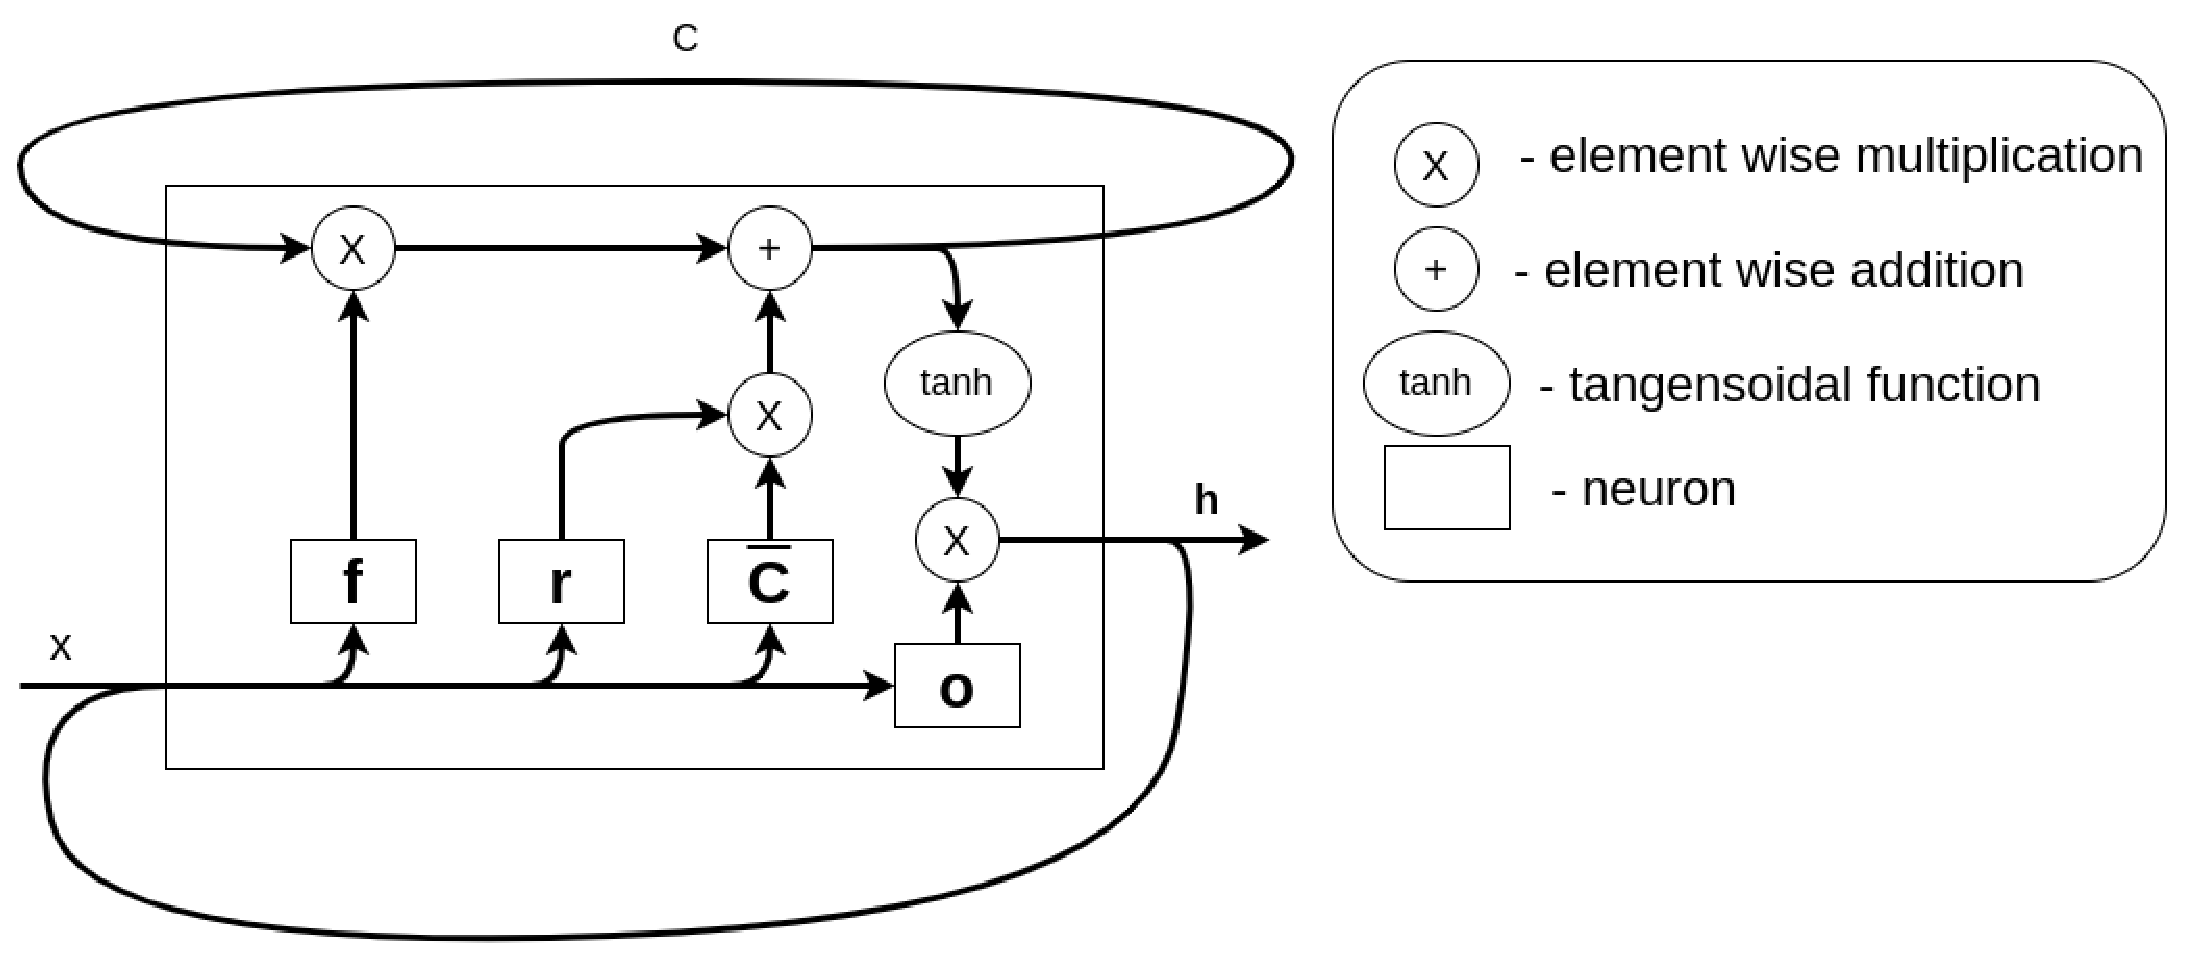
\includegraphics[width=10cm]{res/lstm}
	\caption{LSTM layer}
	\label{fig:lstm}
\end{figure}
Single LSTM neuron consists of four basic neurons and two non-neuron operations:
\begin{itemize}
	\item $x'(t)=[x(t)|h(t-1)]$,
	\item $o_t=\sigma (W_o x'_t+b_o)$,
	\item $r_t=\sigma (W_r x'_t+b_r)$,
	\item $f_t=\sigma (W_f x'_t+b_f)$,
	\item $\bar{C}_t=\tanh (W_c x'_t+b_c)$,
	\item $C_t=f_t\odot C_{t-1}+r_t\odot \bar{C}_t$,
	\item $h_t=o_t\odot \tanh (C_t)$,
\end{itemize}
with $W$ and $b$ being weights and biases for each basic neuron, $x$ input, $y$ output and
$C$ long term memory. As can be seen, $o_t$ is the equivalent of SRU and is moderated by
long term memory before propagating as output. Temporary value of long term memory based
only on current output $\bar{C}_t$ is calculated and then with help of neurons $r$ and $f$
is transformed into its final value.
Neuron $r$ is called remembering gate and influences to what degree temporary long term
a memory from a given cycle affects its final value while $f$ is forgetting gate and
decides the influence of long-term memory from the last cycle on the current one.
Thanks to such implementation our model can learn to detect both long term regularities and 
short term ones.


\chapter{Machine learning in GPS clock bias prediction}


%====================================================================================================
\section{Review of research}

%====================================================================================================
\section{Data overview}

%====================================================================================================
\section{Linear regression baed approach}

%====================================================================================================
\section{Polynomial regression based approach}

%====================================================================================================
\section{Support vector regression based approach}

%====================================================================================================
\section{Neural network based approach}




%----------------------------------------------------------------------------------------
%	BIBLIOGRAPHY
%----------------------------------------------------------------------------------------

\nocite{*}
\printbibliography[heading=bibintoc]

%----------------------------------------------------------------------------------------
%	THESIS CONTENT - APPENDICES
%----------------------------------------------------------------------------------------

\appendix % Cue to tell LaTeX that the following "chapters" are Appendices

% Include the appendices of the thesis as separate files from the Appendices folder
% Uncomment the lines as you write the Appendices

% Appendix A

\chapter{Frequently Asked Questions} % Main appendix title

\label{AppendixA} % For referencing this appendix elsewhere, use \ref{AppendixA}

\section{How do I change the colors of links?}

The color of links can be changed to your liking using:

{\small\verb!\hypersetup{urlcolor=red}!}, or

{\small\verb!\hypersetup{citecolor=green}!}, or

{\small\verb!\hypersetup{allcolor=blue}!}.

\noindent If you want to completely hide the links, you can use:

{\small\verb!\hypersetup{allcolors=.}!}, or even better: 

{\small\verb!\hypersetup{hidelinks}!}.

\noindent If you want to have obvious links in the PDF but not the printed text, use:

{\small\verb!\hypersetup{colorlinks=false}!}.

%\include{Appendices/AppendixB}
%\include{Appendices/AppendixC}

%----------------------------------------------------------------------------------------

\end{document}  
